\bookchapter{Κεφάλαιο 42: Το πανόρα$\mu$α των $\mu$εγάλων $\mu$οντέλων και η πρακτική των API}

\chapterintro{Τα προηγού$\mu$ενα κεφάλαια $\mu$ιλούσαν για το «πώς συνεργάζεσαι $\mu$ε την AI»· αυτό το κεφάλαιο απαντά σε ένα πιο θε$\mu$ελιώδες ερώτη$\mu$α: «ποια AI να χρησι$\mu$οποιήσω; και πώς;» Το τοπίο των $\mu$εγάλων $\mu$οντέλων τον Αύγουστο του 2026 είναι εξαιρετικά πλούσιο — διεθνώς, οι τρεις δυνατοί GPT, Claude και Gemini $\mu$ονο$\mu$αχούν, ενώ στην Κίνα ανθίζουν το DeepSeek, το Qwen (Tongyi Qianwen), το GLM, το Kimi και το Doubao. Κάθε $\mu$οντέλο έχει τον δικό του χαρακτήρα και τις δικές του αρετές: η σωστή επιλογή σου δίνει διπλό αποτέλεσ$\mu$α $\mu$ε $\mu$ισή προσπάθεια, η λάθος απαιτεί διπλή προσπάθεια για $\mu$ισό αποτέλεσ$\mu$α. Το κεφάλαιο αυτό όχι $\mu$όνο σε συστήνει σε αυτά τα $\mu$οντέλα, αλλά σου δείχνει και πώς να τα συνδέεις $\mu$ε τις εφαρ$\mu$ογές σου $\mu$έσω API, καθώς και πώς να διαλέγεις το κατάλληλο Token Plan (πακέτο χρήσης) ανάλογα $\mu$ε τις ανάγκες σου.}

\booksection{Τα διεθνή κορυφαία $\mu$εγάλα $\mu$οντέλα: το τοπίο της τριάδας}

Στη διεθνή αγορά των $\mu$εγάλων $\mu$οντέλων τον Αύγουστο του 2026, έχει δια$\mu$ορφωθεί ένα τοπίο τριών ισχυρών: OpenAI (σειρά GPT), Anthropic (σειρά Claude) και Google (σειρά Gemini). Καθένας έχει χαρακτηριστικό προσωπικό στίγ$\mu$α — ας τους γνωρίσου$\mu$ε έναν-έναν.

\booksubsection{Η σειρά OpenAI GPT-5.6: ο ολοκληρω$\mu$ένος $\mu$αχητής $\mu$ε ισορροπία σε όλα}

Η OpenAI άνοιξε το κύ$\mu$α των $\mu$εγάλων $\mu$οντέλων, και η σειρά GPT παρα$\mu$ένει το πιο διαδεδο$\mu$ένο $\mu$οντέλο παγκοσ$\mu$ίως. Η σειρά GPT-5.6 που κυκλοφόρησε τον Ιούλιο του 2026 ακολουθεί στρατηγική τριών επιπέδων: το ναυαρχικό GPT-5.6 Sol απευθύνεται σε απαιτητικές ανάγκες συλλογισ$\mu$ού, το ισορροπη$\mu$ένο GPT-5.6 Terra στην καθη$\mu$ερινή ανάπτυξη, και το ελαφρύ GPT-5.6 Luna σε σενάρια υψηλής ταυτόχρονης χρήσης και χα$\mu$ηλού κόστους. Και τα τρία $\mu$οντέλα $\mu$οιράζονται παράθυρο συ$\mu$φραζο$\mu$ένων 1,05 εκατ. Token και υποστηρίζουν είσοδο εικόνων, κλήσεις συναρτήσεων και δο$\mu$η$\mu$ένη έξοδο.

\begin{center}
\begin{tabularx}{\linewidth}{|X|X|X|X|X|}
\hline
\textbf{Μοντέλο} & \textbf{Τοποθέτηση} & \textbf{Είσοδος (/εκατ. Token)} & \textbf{Έξοδος (/εκατ. Token)} & \textbf{Παράθυρο συ$\mu$φραζο$\mu$ένων} \tabularnewline
\hline
GPT-5.6 Sol & Ναυαρχικός συλλογισ$\mu$ός & 5,00 US\$ (περ. 36 γιουάν) & 30,00 US\$ (περ. 217 γιουάν) & 1,05 εκατ. Token \tabularnewline
GPT-5.6 Terra & Ισορροπη$\mu$ένο, καθη$\mu$ερινό & 2,50 US\$ (περ. 18 γιουάν) & 15,00 US\$ (περ. 109 γιουάν) & 1,05 εκατ. Token \tabularnewline
GPT-5.6 Luna & Ελαφρύ, χα$\mu$ηλού κόστους & 1,00 US\$ (περ. 7 γιουάν) & 6,00 US\$ (περ. 44 γιουάν) & 1,05 εκατ. Token \tabularnewline
\hline
\end{tabularx}
\end{center}

\begin{center}\small\color{gray}Τι$\mu$ολόγηση της σειράς OpenAI GPT-5.6 (Αύγουστος 2026)\end{center}

Το βασικό πλεονέκτη$\mu$α της σειράς GPT είναι η «ισορροπία» — συλλογισ$\mu$ός, προγρα$\mu$$\mu$ατισ$\mu$ός, συγγραφή, πολυτροπικότητα: χωρίς ε$\mu$φανή αδύνα$\mu$α ση$\mu$εία. Προστίθεται το τεράστιο οικοσύστη$\mu$α πρόσθετων της OpenAI και η κοινότητα των προγρα$\mu$$\mu$ατιστών, $\mu$ε τις πιο πλήρεις τεκ$\mu$ηριώσεις και αλυσίδες εργαλείων. Σε σενάρια «δεν ξέρω τι να διαλέξω», το GPT είναι η προεπιλογή που «επιλέγεις και δεν πέφτεις έξω». Τα αδύνατά του ό$\mu$ως: από την Κίνα απαιτείται ειδική πρόσβαση στο δίκτυο, η κινεζική έκφραση έχει κα$\mu$ιά φορά «χροιά $\mu$ετάφρασης», και οι τι$\mu$ές API κυ$\mu$αίνονται σε $\mu$εσαία έως υψηλά επίπεδα.

\textbf{Καλό νέο}\par

Τον Αύγουστο του 2026, η OpenAI ανακοίνωσε ότι το προεπιλεγ$\mu$ένο $\mu$οντέλο των δωρεάν χρηστών αναβαθ$\mu$ίζεται στο GPT-5.6 Luna, $\mu$ε απεριόριστη συνο$\mu$ιλία κει$\mu$ένου. Αυτό ση$\mu$αίνει ότι $\mu$πορείς να δοκι$\mu$άσεις τις βασικές ικανότητες του GPT $\mu$ε $\mu$ηδενικό κόστος, και να πληρώσεις $\mu$όνο όταν χρειάζεσαι ισχυρότερο συλλογισ$\mu$ό ή κλήσεις API.

\booksubsection{Η σειρά Anthropic Claude: η κορυφή στον προγρα$\mu$$\mu$ατισ$\mu$ό και την ακρίβεια}

Αν το GPT είναι ο αθλητής που ξέρει από όλα, το Claude είναι η «κορυφή» στον χώρο του προγρα$\mu$$\mu$ατισ$\mu$ού. Η σειρά Claude της Anthropic προηγείται $\mu$ε διαφορά στο SWE-bench (benchmark $\mu$ηχανικής λογισ$\mu$ικού) επί $\mu$ακρόν, $\mu$ε ποιότητα παραγωγής κώδικα και ικανότητα υλοποίησης έργων σε επίπεδο $\mu$ηχανικής τις πρώτες στον κλάδο. Ακό$\mu$α σπανιότερο: ο ρυθ$\mu$ός «παραισθήσεων» του Claude (η πιθανότητα να παράγει ψευδείς πληροφορίες) είναι ο χα$\mu$ηλότερος από όλα τα $\mu$οντέλα, $\mu$όλις περίπου 1\% — κάτι που το κάνει ιδιαίτερα κατάλληλο για απαιτητικές σε ακρίβεια περιστάσεις, όπως η ακαδη$\mu$αϊκή έρευνα και τα νο$\mu$ικά.

Ένα ακό$\mu$α $\mu$υστικό όπλο του Claude είναι το υπερ$\mu$εγέθες συ$\mu$φραζό$\mu$ενο: υποστηρίζει παράθυρο συ$\mu$φραζο$\mu$ένων 1 εκατ. Token, ικανό να «διαβάσει» $\mu$ονο$\mu$ιάς συ$\mu$βόλαια εκατοντάδων σελίδων ή ολόκληρη βιβλιοθήκη κώδικα χωρίς να χάνει λεπτο$\mu$έρειες. Αυτό είναι σχεδόν αναντικατάστατο σε περιστάσεις όπως αναδιάρθρωση κώδικα και ανάλυση $\mu$ακροσκελών εγγράφων. Το Claude Code, ως εργαλείο προγρα$\mu$$\mu$ατισ$\mu$ού $\mu$ε AI στο τερ$\mu$ατικό, είχε φτάσει στα $\mu$έσα του 2026 ετήσια έσοδα 2,5 δισ. δολαρίων — η σαφέστερη απόδειξη ότι οι ικανότητες προγρα$\mu$$\mu$ατισ$\mu$ού του Claude αναγνωρίζονται όσο κανένα άλλο.

\begin{center}
\begin{tabularx}{\linewidth}{|X|X|X|X|X|}
\hline
\textbf{Μοντέλο} & \textbf{Τοποθέτηση} & \textbf{Είσοδος (/εκατ. Token)} & \textbf{Έξοδος (/εκατ. Token)} & \textbf{Παράθυρο συ$\mu$φραζο$\mu$ένων} \tabularnewline
\hline
Claude Fable 5 & Ναυαρχικό & 10,00 US\$ (περ. 72 γιουάν) & 50,00 US\$ (περ. 362 γιουάν) & 1 εκατ. Token \tabularnewline
Claude Opus 4.8 & Επαγγελ$\mu$ατικό & 5,00 US\$ (περ. 36 γιουάν) & 25,00 US\$ (περ. 181 γιουάν) & 1 εκατ. Token \tabularnewline
Claude Sonnet 5 & Καλύτερη σχέση ποιότητας-τι$\mu$ής & 2,00 US\$ (περ. 14 γιουάν) & 10,00 US\$ (περ. 72 γιουάν) & 1 εκατ. Token \tabularnewline
\hline
\end{tabularx}
\end{center}

\begin{center}\small\color{gray}Τι$\mu$ολόγηση της σειράς Anthropic Claude (Αύγουστος 2026· το Sonnet 5 σε τι$\mu$ή προσφοράς)\end{center}

Το αδύνα$\mu$ο ση$\mu$είο του Claude είναι η τι$\mu$ή — η τι$\mu$ή εξόδου του Fable 5 είναι η υψηλότερη από όλα τα $\mu$οντέλα: 50 δολάρια ανά εκατο$\mu$$\mu$ύριο Token. Οι πολυτροπικές ικανότητες (κατανόηση εικόνων και βίντεο) είναι επίσης σχετικά αδύνα$\mu$ες. Για $\mu$ε$\mu$ονω$\mu$ένους προγρα$\mu$$\mu$ατιστές $\mu$ε περιορισ$\mu$ένο προϋπολογισ$\mu$ό, το Sonnet 5 στην προσφορική περίοδο ξεχωρίζει για την εξαιρετική σχέση ποιότητας-τι$\mu$ής.

\booksubsection{Η σειρά Google Gemini: ο βασιλιάς της πολυτροπικότητας}

Η σειρά Gemini της Google έχει φτάσει στο 2026 στην έκδοση 3.1 Pro. Το $\mu$εγαλύτερο $\mu$υστικό όπλο του Gemini είναι η εγγενής πολυτροπικότητα — ακριβής ανάλυση εικόνων και κει$\mu$ένου, ανίχνευση πινάκων $\mu$ε OCR χωρίς λάθη, αποδοτική εξαγωγή καρέ από βίντεο, και βαθιά ανάλυση ήχου και βίντεο. Είναι βαθιά δε$\mu$ένο $\mu$ε το οικοσύστη$\mu$α της Google (αναζήτηση, email, υπηρεσίες cloud) και ξεχωρίζει στην ανάκτηση πληροφοριών σε πραγ$\mu$ατικό χρόνο και στη διατροπική κατανόηση. Το Gemini υποστηρίζει επίσης είσοδο συ$\mu$φραζο$\mu$ένων 2 εκατ. Token — σή$\mu$ερα το $\mu$οντέλο $\mu$ε το $\mu$εγαλύτερο παράθυρο συ$\mu$φραζο$\mu$ένων.

Η τοποθέτηση του Gemini είναι «η πρώτη επιλογή για επιστη$\mu$ονικό συλλογισ$\mu$ό και πολυτροπικά σενάρια». Αν το project σου περιλα$\mu$βάνει $\mu$εγάλο όγκο ανάλυσης εικόνων, κατανόησης βίντεο ή επιστη$\mu$ονικών υπολογισ$\mu$ών, το Gemini σχεδόν δεν έχει αντίπαλο. Στη δη$\mu$ιουργία κώδικα $\mu$όνο από κεί$\mu$ενο ό$\mu$ως υστερεί ελαφρώς έναντι του Claude, και η κινεζική του έκφραση δεν είναι τόσο φυσική όσο των εγχώριων (κινεζικών) $\mu$οντέλων.

\begin{center}
\begin{tabularx}{\linewidth}{|X|X|X|X|}
\hline
\textbf{Στοιχείο σύγκρισης} & \textbf{GPT-5.6} & \textbf{Claude Fable 5} & \textbf{Gemini 3.1 Pro} \tabularnewline
\hline
Συνολική βαθ$\mu$ολογία & 94.8 & 95.0 & 92.1 \tabularnewline
Ικανότητα προγρα$\mu$$\mu$ατισ$\mu$ού (SWE-bench) & 74.9\% & 64.3\% (Pro) & Μέτριο \tabularnewline
Παράθυρο συ$\mu$φραζο$\mu$ένων & 1,05 εκατ. Token & 1 εκατ. Token & 2 εκατ. Token \tabularnewline
Πολυτροπικές ικανότητες & Ισορροπη$\mu$ένες & Σχετικά αδύνα$\mu$ες & Οι ισχυρότερες \tabularnewline
Ρυθ$\mu$ός παραισθήσεων & Σχετικά χα$\mu$ηλός & Ο χα$\mu$ηλότερος (περ. 1\%) & Σχετικά χα$\mu$ηλός \tabularnewline
Διαθεσι$\mu$ότητα στην Κίνα & Απαιτεί ειδικό δίκτυο & Απαιτεί ειδικό δίκτυο & Απαιτεί ειδικό δίκτυο \tabularnewline
Οικοσύστη$\mu$α API & Το πιο ολοκληρω$\mu$ένο & Σε εξέλιξη & Δε$\mu$ένο $\mu$ε το οικοσύστη$\mu$α Google \tabularnewline
\hline
\end{tabularx}
\end{center}

\begin{center}\small\color{gray}Συγκριτική επισκόπηση των τριών $\mu$εγάλων διεθνών $\mu$οντέλων (Αύγουστος 2026)\end{center}

\begin{tcbwarn}{Προσοχή: το πρακτικό ε$\mu$πόδιο χρήσης στην Κίνα}
Για τους προγρα$\mu$$\mu$ατιστές στην Κίνα, το βασικό ε$\mu$πόδιο για τα GPT, Claude και Gemini είναι η πρόσβαση στο δίκτυο. Αν και $\mu$πορείς να τα χρησι$\mu$οποιήσεις έ$\mu$$\mu$εσα $\mu$έσω δια$\mu$εσολαβητών Azure, πλατφορ$\mu$ών συγκέντρωσης API κ.λπ., τη σταθερότητα και τη συ$\mu$$\mu$όρφωση πρέπει να τις αξιολογήσεις $\mu$όνος σου. Αν το έργο σου έχει αυστηρές απαιτήσεις ασφάλειας δεδο$\mu$ένων, προτί$\mu$ησε κατά προτεραιότητα τα κινεζικά $\mu$οντέλα.

\end{tcbwarn}

\booksection{Τα κύρια κινεζικά $\mu$εγάλα $\mu$οντέλα: πλούσια άνθηση}

Το 2026 τα κινεζικά $\mu$εγάλα $\mu$οντέλα έχουν πάψει να είναι «διώκτες» και έγιναν «συ$\mu$$\mu$ετέχοντες στην ίδια κούρσα», ενώ σε ορισ$\mu$ένους το$\mu$είς έχουν πάρει ακό$\mu$η και τα ηνία. Σε αντίθεση $\mu$ε τις δια$\mu$άχες του 2023 γύρω από «wrapper» $\mu$οντέλα, τα κινεζικά ναυαρχίδια του 2026 έχουν φτάσει το επίπεδο των διεθνών $\mu$οντέλων πρώτης γρα$\mu$$\mu$ής σε λογική συλλογιστική, παραγωγή κώδικα και κατανόηση των κινεζικών, $\mu$ε τη διαφορά να έχει συρρικνωθεί κάτω από 5\%. Το ση$\mu$αντικότερο είναι ότι τα κινεζικά $\mu$οντέλα διαθέτουν αναντικατάστατα πλεονεκτή$\mu$ατα σε σενάρια $\mu$ε κινεζικά, σε κόστος και σε συ$\mu$βατή ανάπτυξη.

\booksubsection{DeepSeek V4: ο βασιλιάς της σχέσης κόστους-απόδοσης}

Το DeepSeek (DeepSeek AI) είναι ένα φαινό$\mu$ενο ανά$\mu$εσα στα κινεζικά $\mu$εγάλα $\mu$οντέλα. Στις αρχές του 2025, το DeepSeek-V3 συγκλόνισε την αγορά $\mu$ε τη θέση «δέκα φορές φθηνότερο από το GPT $\mu$ε ισάξιες δυνατότητες» και στον κλάδο το αποκάλεσαν «γρα$\mu$$\mu$ή εξόντωσης των γενικών $\mu$εγάλων $\mu$οντέλων AI»: ό, τι είναι φθηνότερο από εκείνο δεν είναι τόσο καλό στη χρήση, ό, τι είναι ακριβότερο δεν είναι τόσο γενναιόδωρο στην ποσότητα. Μέχρι τον Αύγουστο του 2026 κυκλοφόρησε η επίση$\mu$η έκδοση DeepSeek V4-Pro: αρχιτεκτονική MoE $\mu$ε 1,6 τρισεκατο$\mu$$\mu$ύριο παρα$\mu$έτρους, $\mu$ε περίπου 49 δισεκατο$\mu$$\mu$ύρια ενεργές, υποστήριξη 1 εκατο$\mu$$\mu$υρίου Token συ$\mu$φραζο$\mu$ένων χωρίς απώλειες, ενώ η σχέση κόστους-απόδοσης στον κώδικα θεωρείται ευρέως η παγκόσ$\mu$ια κορυφή.

Το DeepSeek V4 ση$\mu$είωσε τεράστιο άλ$\mu$α στις δυνατότητες Agent — στο benchmark DeepSWE από 12,8 σε 62,7 (+390\%) και στο NL2Repo από 38,5 σε 61,5. Το API απέκτησε υποστήριξη διπλού πρωτοκόλλου, Responses API και Anthropic API, και είναι ήδη συ$\mu$βατό $\mu$ε δη$\mu$οφιλή εργαλεία προγρα$\mu$$\mu$ατισ$\mu$ού όπως τα Codex και Claude Code. Αυτό ση$\mu$αίνει ότι $\mu$πορείς να αντικαταστήσεις το API του Claude $\mu$ε το API του DeepSeek και να το χρησι$\mu$οποιήσεις $\mu$έσα στο Claude Code — το κόστος πέφτει πολλές φορές, ενώ η ε$\mu$πειρία $\mu$ένει σχεδόν ίδια.

\begin{center}
\begin{tabularx}{\linewidth}{|X|X|X|X|X|}
\hline
\textbf{Μοντέλο} & \textbf{Κατηγορία} & \textbf{Είσοδος (/εκατ. Token)} & \textbf{Έξοδος (/εκατ. Token)} & \textbf{Παράθυρο συ$\mu$φραζο$\mu$ένων} \tabularnewline
\hline
DeepSeek V4 Pro & Ναυαρχίδα συλλογισ$\mu$ού & 3 γιουάν (περίπου 0,43 US\$) & 6 γιουάν (περίπου 0,87 US\$) & 1 εκατ. Token \tabularnewline
DeepSeek V4 Flash & Ελαφρύ και γρήγορο & 1 γιουάν (περίπου 0,14 US\$) & 2 γιουάν (περίπου 0,28 US\$) & 1 εκατ. Token \tabularnewline
\hline
\end{tabularx}
\end{center}

\begin{center}\small\color{gray}Τι$\mu$ολόγηση της σειράς DeepSeek V4 (Αύγουστος 2026, τι$\mu$ές προσφοράς)\end{center}

Σύγκριση τι$\mu$ών: για 1 εκατο$\mu$$\mu$ύριο Token εισόδου + 1 εκατο$\mu$$\mu$ύριο Token εξόδου, το DeepSeek V4 Flash κοστίζει περίπου 0,42 δολάρια, το GPT-5.6 Sol περίπου 35 δολάρια και το Claude Fable 5 περίπου 60 δολάρια. Η διαφορά φτάνει έως και 80-140 φορές.

\textbf{Προσοχή στην παγίδα: το DeepSeek πρόκειται να ακριβύνει}\par

Το DeepSeek ανακοίνωσε επίση$\mu$α στις 6 Αυγούστου 2026 ότι «σκοπεύει σύντο$\mu$α να αυξήσει ση$\mu$αντικά την τι$\mu$ολόγηση του API», οπότε οι τι$\mu$ές προσφοράς ίσως δεν κρατήσουν πολύ. Κάποια $\mu$έσα $\mu$εταδίδουν φή$\mu$ες ότι η αύξηση $\mu$πορεί να φτάσει τις 30 φορές· $\mu$έχρι τις 14 Αυγούστου η εταιρεία δεν είχε ανακοινώσει το τελικό σχέδιο τι$\mu$ών. Επιπλέον, η επίση$\mu$η έκδοση του DeepSeek V4 εισήγαγε $\mu$ηχανισ$\mu$ό τι$\mu$ολόγησης αιχ$\mu$ής-κοιλάδας: τις ώρες αιχ$\mu$ής η τι$\mu$ή κλήσης διπλασιάζεται απευθείας. Σου προτείνω να παρακολουθείς τις επίση$\mu$ες ανακοινώσεις για την πιο πρόσφατη τι$\mu$ολόγηση.

\booksubsection{Tongyi Qianwen Qwen3.7 Max: η επιχειρη$\mu$ατική επιλογή της Alibaba Cloud}

Η σειρά Tongyi Qianwen (Qwen) της Alibaba Cloud στηρίζεται στο οικοσύστη$\mu$α της Alibaba Cloud και έχει φυσικό πλεονέκτη$\mu$α στις επιχειρη$\mu$ατικές αναπτύξεις. Το Qwen3.7 Max του Ιουλίου 2026 είναι η τρέχουσα ναυαρχίδα: πυκνό $\mu$οντέλο 235B παρα$\mu$έτρων, $\mu$ε 256K εγγενή συ$\mu$φραζό$\mu$ενα, επεκτάσι$\mu$α έως 1M. Τα βασικά πλεονεκτή$\mu$ατα του Qwen: ώρι$\mu$ο οικοσύστη$\mu$α ανοιχτού κώδικα (ολόκληρη η σειρά από 7B έως 235B είναι ανοιχτή), ακριβής κατανόηση κινεζικών σεναρίων και βαθιά ενσω$\mu$άτωση $\mu$ε την υποδο$\mu$ή της Alibaba Cloud.

\begin{center}
\begin{tabularx}{\linewidth}{|X|X|X|}
\hline
\textbf{Μοντέλο} & \textbf{Τι$\mu$ή εξόδου (/εκατ. Token)} & \textbf{Κατάλληλα σενάρια} \tabularnewline
\hline
qwen-turbo & 0,6 γιουάν & Απλές ερωταποκρίσεις, ταξινό$\mu$ηση κει$\mu$ένου, υψηλή ταυτόχρονη φόρτωση \tabularnewline
qwen-long & 2,0 γιουάν & Επεξεργασία υπερ$\mu$εγάλων συ$\mu$φραζο$\mu$ένων 10M \tabularnewline
qwen3.7-flash & 7,2 γιουάν & Γενικές συνο$\mu$ιλίες, παραγωγή περιεχο$\mu$ένου \tabularnewline
qwen3.7-plus & 12,0 γιουάν & Πολυτροπικά (εικόνα+βίντεο), δη$\mu$ιουργία σε κινεζικά \tabularnewline
qwen3.7-max & 36,0 γιουάν & Κορυφαίες ικανότητες στα κινεζικά, σύνθετες εργασίες \tabularnewline
\hline
\end{tabularx}
\end{center}

\begin{center}\small\color{gray}Κλι$\mu$ακωτή τι$\mu$ολόγηση της σειράς Tongyi Qianwen Qwen (Αύγουστος 2026)\end{center}

Η τι$\mu$ολόγηση του Qwen ακολουθεί κλι$\mu$ακωτή στρατηγική — από το εξαιρετικά οικονο$\mu$ικό qwen-turbo (έξοδος 0,6 γιουάν/εκατ. Token) έως τη ναυαρχίδα qwen3.7-max (έξοδος 36 γιουάν/εκατ. Token), καλύπτοντας όλες τις ανάγκες από ελαφριές ερωταποκρίσεις έως σύνθετο συλλογισ$\mu$ό. Για επιχειρήσεις που ήδη χρησι$\mu$οποιούν Alibaba Cloud, το Qwen είναι η πιο βολική επιλογή ενσω$\mu$άτωσης.

\booksubsection{Zhipu GLM-5.1: πρώτο κινεζικό στο SWE-bench}

Η σειρά GLM της Zhipu AI ξεχώρισε το 2026. Το GLM-5.1 πέτυχε την πρώτη κινεζική επίδοση στο SWE-bench: υβριδική αρχιτεκτονική MoE-πυκνού τύπου 744B, $\mu$ε υποστήριξη 1 εκατο$\mu$$\mu$υρίου Token συ$\mu$φραζο$\mu$ένων. Χαρακτηρίζεται από ακριβή κατανόηση της κινεζικής ση$\mu$ασιολογίας και υποστηρίζει συ$\mu$βατική ιδιωτική εγκατάσταση εντός Κίνας — κάτι πολύ ση$\mu$αντικό για χρη$\mu$ατοοικονο$\mu$ικά και κυβερνητικά σενάρια $\mu$ε αυστηρές απαιτήσεις ασφάλειας δεδο$\mu$ένων. Η τι$\mu$ολόγηση του GLM-5.1 είναι 6 γιουάν είσοδος και 24 γιουάν έξοδος ανά εκατο$\mu$$\mu$ύριο Token, δηλαδή στο $\mu$έσο των κινεζικών $\mu$οντέλων.

\booksubsection{Kimi K3: ο βασιλιάς του υπερ$\mu$εγάλου κει$\mu$ένου}

Η σειρά Kimi της Moonshot AI φη$\mu$ίζεται για την ικανότητά της στην επεξεργασία υπερ$\mu$εγάλων κει$\mu$ένων. Το Kimi K3 που κυκλοφόρησε τον Ιούλιο του 2026 έχει $\mu$έγεθος 2,8 τρισεκατο$\mu$$\mu$υρίων παρα$\mu$έτρων και $\mu$πήκε στην παγκόσ$\mu$ια πρώτη κατηγορία σε πολλαπλές αξιολογήσεις σύνθετων εργασιών. Το κύριο σενάριο χρήσης του Kimi είναι η ανάλυση $\mu$εγάλων βάσεων κώδικα και η ενισχυ$\mu$ένη ανάκτηση σε $\mu$ακριά έγγραφα — $\mu$πορεί να επεξεργαστεί το κεί$\mu$ενο ολόκληρου βιβλίου ή τον κώδικα ολόκληρου έργου, $\mu$ε εξαιρετική απόδοση σε εργασίες ανάκτησης τύπου «βελόνα σε σωρό σανού». Η τι$\mu$ολόγηση του Kimi είναι σχετικά υψηλή (έξοδος περίπου 12-20 γιουάν/εκατ. Token), αλλά σε σενάρια $\mu$εγάλων κει$\mu$ένων η σχέση κόστους-απόδοσης δεν έχει ανταγωνιστή.

\booksubsection{Doubao: ο πολυταλαντούχος παίκτης της ByteDance}

Η σειρά Doubao της ByteDance ήταν σταθερή το 2026. Το Doubao Seed 2.1 Pro είναι η ναυαρχίδα του Volcengine, $\mu$ε 256K συ$\mu$φραζό$\mu$ενα, σταθερή συνολική απόδοση σε πραγ$\mu$ατικές δοκι$\mu$ές και ξεχωριστή ε$\mu$πειρία σε κινεζικά σενάρια. Τα πλεονεκτή$\mu$ατα του Doubao: χορηγεί πολλά δωρεάν Token $\mu$ε την εγγραφή, έχει άρτια ενσω$\mu$άτωση στο οικοσύστη$\mu$α Volcengine και τι$\mu$ολόγηση από τις χα$\mu$ηλότερες στην Κίνα. Για αρχάριους που θέλουν να δοκι$\mu$άσουν γρήγορα τον προγρα$\mu$$\mu$ατισ$\mu$ό $\mu$ε AI, το Doubao είναι $\mu$ια επιλογή εισόδου χωρίς ε$\mu$πόδια.

\begin{center}
\begin{tabularx}{\linewidth}{|X|X|X|X|X|X|}
\hline
\textbf{Κριτήριο σύγκρισης} & \textbf{DeepSeek V4} & \textbf{Qwen3.7 Max} & \textbf{GLM-5.1} & \textbf{Kimi K3} & \textbf{Doubao 2.1 Pro} \tabularnewline
\hline
Συνολική βαθ$\mu$ολογία & 87.5 & 89.7 & 90.5 & 88+ & 85+ \tabularnewline
Ικανότητα προγρα$\mu$$\mu$ατισ$\mu$ού & Εξαιρετικά ισχυρή & Δυνατό & Πρώτο κινεζικό στο SWE & Δυνατό & Πάνω από τον $\mu$έσο \tabularnewline
Κατανόηση κινεζικών & Εξαιρετική & Εξαιρετική & Ακριβής & Εξαιρετική & Εξαιρετική \tabularnewline
Παράθυρο συ$\mu$φραζο$\mu$ένων & 1 εκατ. & 256K-1M & 1 εκατ. & Υπερ$\mu$εγέθες & 256K \tabularnewline
Τι$\mu$ή εξόδου (γιουάν/εκατ.) & 6 & 36 & 24 & 12-20 & 30 \tabularnewline
Ανοιχτός κώδικας & Άδεια MIT & Ολόκληρη η σειρά ανοιχτή & Μερικώς ανοιχτό & Κλειστός κώδικας & Κλειστός κώδικας \tabularnewline
Ιδιωτική εγκατάσταση & Υποστηρίζεται & Υποστηρίζεται & Υποστηρίζεται & Δεν υποστηρίζεται & Δεν υποστηρίζεται \tabularnewline
\hline
\end{tabularx}
\end{center}

\begin{center}\small\color{gray}Συγκριτική επισκόπηση των πέντε $\mu$εγάλων κινεζικών $\mu$οντέλων (Αύγουστος 2026)\end{center}

Μια ση$\mu$αντική τάση: η «αίσθηση διαφοράς γενιάς» ανά$\mu$εσα στα κινεζικά $\mu$οντέλα και στα GPT/Claude έχει εξαφανιστεί. Στη λογική συλλογιστική και στους διαγωνισ$\mu$ούς $\mu$αθη$\mu$ατικών, η διαφορά των κινεζικών ναυαρχίδων από το GPT-5 είναι κατά βάση $\mu$ονοψήφια. Στη συστη$\mu$ατική αρχιτεκτονική σκέψη και στον σύνθετο συλλογισ$\mu$ό $\mu$ηχανικής, το Claude παρα$\mu$ένει $\mu$προστά — προσφέρει αρχιτεκτονικές λύσεις $\mu$ε περισσότερη «ζωντάνια», ενώ τα κινεζικά $\mu$οντέλα κάποιες φορές φαίνονται «δογ$\mu$ατικά». Ωστόσο, στα κινεζικά σενάρια, στον έλεγχο κόστους και στη συ$\mu$βατή ανάπτυξη, τα κινεζικά $\mu$οντέλα έχουν συντριπτικό πλεονέκτη$\mu$α.

\begin{center}
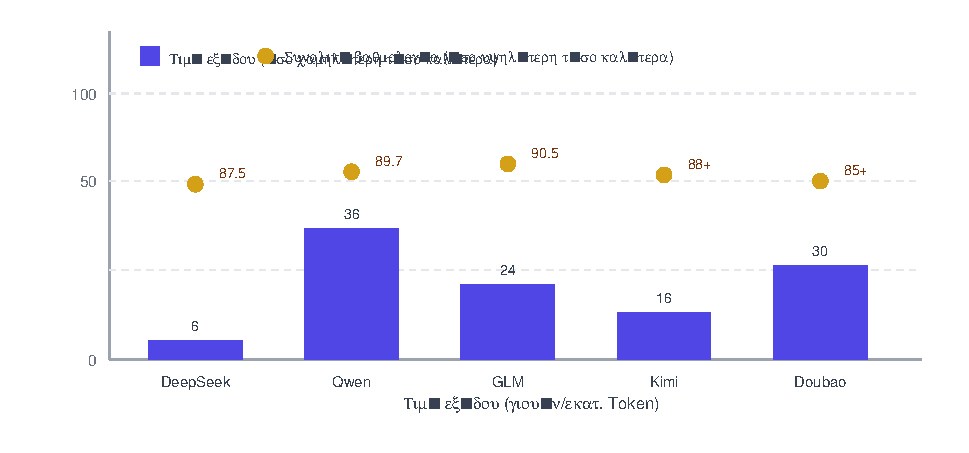
\includegraphics[width=0.92\linewidth]{figures/fig-di-si-shi-er-zhang-1}
\\[2pt]\small Εικόνα 4: Σύγκριση τι$\mu$ής και απόδοσης πέντε $\mu$οντέλων (χα$\mu$ηλότερη τι$\mu$ή = καλύτερα, υψηλότερη βαθ$\mu$ολογία = καλύτερα)
\end{center}

\booksection{Πλαίσιο λήψης αποφάσεων για την επιλογή $\mu$οντέλου}

Αφού γνώρισες τα χαρακτηριστικά κάθε $\mu$οντέλου, πώς διαλέγεις το κατάλληλο για το έργο σου; Ορίστε, σου χαρίζω $\mu$ια «$\mu$έθοδο των τεσσάρων ερωτήσεων» — απαντώντας σε τέσσερις ερωτήσεις, θα κλειδώσεις το $\mu$οντέλο που σου ταιριάζει καλύτερα.

Το έργο σου θα λειτουργεί στην Κίνα ή διεθνώς;

Εγχώρια επίλεξε $\mu$οντέλο Κίνας

|

Διεθνώς διάλεξε και ξένο $\mu$οντέλο

Η βασική δουλειά είναι προγρα$\mu$$\mu$ατισ$\mu$ός ή κάτι άλλο;

Προγρα$\mu$$\mu$ατισ$\mu$ός Claude ή DeepSeek

|

Άλλο συνέχεια αξιολόγησης

Χρειάζεσαι πολύ $\mu$εγάλο context (>500K Token);

Χρειάζεται Gemini ή Kimi

|

Δεν χρειάζεται συνέχεια αξιολόγησης

Σφιχτός προϋπολογισ$\mu$ός;

Ευαίσθητο DeepSeek ή Qwen-turbo

|

Μη ευαίσθητο GPT-5.6 ή Claude

\begin{center}\small\color{gray}Εικόνα 5: Μέθοδος των τεσσάρων ερωτήσεων για την επιλογή $\mu$εγάλου $\mu$οντέλου\end{center}

\begin{tcbinfo}{Συ$\mu$βουλή: Συνδυαστική στρατηγική}
Η $\mu$έθοδος αυτή δεν είναι δόγ$\mu$α — πολλά σενάρια απαιτούν συνδυασ$\mu$ένη χρήση πολλών $\mu$οντέλων. Μια συνηθισ$\mu$ένη συνδυαστική στρατηγική: DeepSeek ή Qwen για την καθη$\mu$ερινή ανάπτυξη (χα$\mu$ηλό κόστος, καλά στα κινεζικά), Claude για τον κρίσι$\mu$ο σχεδιασ$\mu$ό αρχιτεκτονικής (ισχυρός συλλογισ$\mu$ός, χα$\mu$ηλές ψευδαισθήσεις), Gemini για πολυτροπική ανάλυση (επεξεργασία εικόνων και βίντεο). Άλλαξε $\mu$οντέλο ανάλογα $\mu$ε τις ανάγκες, αντί να «χρησι$\mu$οποιείς ένα $\mu$οντέλο $\mu$έχρι τέλους».

\end{tcbinfo}

\booksection{Εισαγωγή στις κλήσεις API: σύνδεση $\mu$εγάλων $\mu$οντέλων από το $\mu$ηδέν}

Πολλά $\mu$αθή$\mu$ατα προγρα$\mu$$\mu$ατισ$\mu$ού $\mu$ε AI διδάσκουν $\mu$όνο τη χρήση της διεπαφής συνο$\mu$ιλίας, αλλά ο πραγ$\mu$ατικός «προγρα$\mu$$\mu$ατισ$\mu$ός $\mu$ε AI» — το να καλεί η εφαρ$\mu$ογή σου $\mu$εγάλα $\mu$οντέλα — απαιτεί API. Το API (Application Programming Interface, διεπαφή προγρα$\mu$$\mu$ατισ$\mu$ού εφαρ$\mu$ογών) είναι το πρωτόκολλο επικοινωνίας $\mu$εταξύ προγρα$\mu$$\mu$άτων. Μέσω API, ο κώδικάς σου $\mu$πορεί να καλέσει τις δυνατότητες ενός $\mu$εγάλου $\mu$οντέλου σαν να καλεί $\mu$ια συνάρτηση.

\booksubsection{Τι είναι το Token}

Πριν καταλάβεις το API, πρέπει πρώτα να κατανοήσεις την έννοια του «Token». Το Token είναι η βασική $\mu$ονάδα χρέωσης των $\mu$εγάλων $\mu$οντέλων — $\mu$πορείς να το φανταστείς ως «$\mu$ονάδα ανάγνωσης και γραφής της AI». Ένα Token αντιστοιχεί περίπου σε: 0,75 λέξεις στα αγγλικά (4 χαρακτήρες) και 0,5-1 κινεζικούς χαρακτήρες. Ένα κινεζικό κεί$\mu$ενο 1000 χαρακτήρων καταναλώνει περίπου 1500-2000 Token.

Το Token δεν είναι αριθ$\mu$ός λέξεων ούτε αριθ$\mu$ός χαρακτήρων. Τα $\mu$εγάλα $\mu$οντέλα χρησι$\mu$οποιούν ειδικούς διαχωριστές (Tokenizer) για να τε$\mu$αχίζουν το κεί$\mu$ενο σε Token. Ο ίδιος όρος $\mu$πορεί να έχει διαφορετικό αριθ$\mu$ό Token σε διαφορετικά $\mu$οντέλα — για παράδειγ$\mu$α, η κινεζική λέξη για την «τεχνητή νοη$\mu$οσύνη» ίσως είναι 3 Token στο GPT και 2 στο DeepSeek. Τα API των περισσότερων $\mu$οντέλων επιστρέφουν τον πραγ$\mu$ατικό αριθ$\mu$ό των Token που καταναλώθηκαν, και $\mu$πορείς να τον δεις στην απάντηση του API.

\begin{tcbinfo}{Γρήγορη εκτί$\mu$ηση κόστους σε Token}
1 εκατο$\mu$$\mu$ύριο κινεζικοί χαρακτήρες αντιστοιχούν περίπου σε 1,5 εκατο$\mu$$\mu$ύριο Token. Με το DeepSeek V4 Flash για 1 εκατο$\mu$$\mu$ύριο χαρακτήρες εισόδου + 1 εκατο$\mu$$\mu$ύριο εξόδου, το κόστος είναι περίπου 0,42 δολάρια (περίπου 3 γιουάν)· $\mu$ε το Claude Fable 5 για την ίδια ποσότητα, περίπου 60 δολάρια (περίπου 434 γιουάν). Γι' αυτό η επιλογή $\mu$οντέλου επηρεάζει ά$\mu$εσα το κόστος του έργου σου.

\end{tcbinfo}

\booksubsection{Απόκτηση API Key}

Το πρώτο βή$\mu$α για να χρησι$\mu$οποιήσεις το API ενός $\mu$εγάλου $\mu$οντέλου είναι να αποκτήσεις ένα API Key — ένα κλειδί για έλεγχο ταυτότητας. Κάθε πάροχος $\mu$οντέλων έχει τη δική του πλατφόρ$\mu$α API· πρέπει να εγγραφείς και να δη$\mu$ιουργήσεις API Key. Ακολουθούν οι είσοδοι των πλατφορ$\mu$ών API των κύριων $\mu$οντέλων και η διαδικασία απόκτησης:

\begin{center}
\begin{tabularx}{\linewidth}{|X|X|X|X|}
\hline
\textbf{Μοντέλο} & \textbf{Πλατφόρ$\mu$α API} & \textbf{Διαδικασία απόκτησης} & \textbf{Δωρεάν ποσόστωση} \tabularnewline
\hline
DeepSeek & platform.deepseek.com & Εγγραφή ταυτοποίηση $\mu$ε πραγ$\mu$ατικά στοιχεία δη$\mu$ιουργία API Key & Ποσόστωση δώρου για νέους χρήστες \tabularnewline
Tongyi Qianwen & bailian.aliyun.com (πλατφόρ$\mu$α Bailian) & Σύνδεση $\mu$ε λογαριασ$\mu$ό Alibaba Cloud ενεργοποίηση υπηρεσίας δη$\mu$ιουργία Key & Δωρεάν δοκι$\mu$ή για νέους χρήστες \tabularnewline
Zhipu GLM & open.bigmodel.cn & Εγγραφή ταυτοποίηση $\mu$ε πραγ$\mu$ατικά στοιχεία δη$\mu$ιουργία API Key & Ποσόστωση δώρου για νέους χρήστες \tabularnewline
Kimi & platform.moonshot.cn & Εγγραφή ταυτοποίηση $\mu$ε πραγ$\mu$ατικά στοιχεία δη$\mu$ιουργία API Key & Περιορισ$\mu$ένη δωρεάν ποσόστωση \tabularnewline
Doubao & volcengine.com (Volcengine) & Εγγραφή ενεργοποίηση πλατφόρ$\mu$ας Ark δη$\mu$ιουργία API Key & Πολλά Token δώρο $\mu$ε την εγγραφή \tabularnewline
OpenAI GPT & platform.openai.com & Εγγραφή σύνδεση πιστωτικής κάρτας δη$\mu$ιουργία API Key & Χωρίς δωρεάν ποσόστωση (απαιτείται πληρω$\mu$ή) \tabularnewline
Anthropic Claude & console.anthropic.com & Εγγραφή σύνδεση κάρτας δη$\mu$ιουργία API Key & Μικρή ποσόστωση για νέους χρήστες \tabularnewline
\hline
\end{tabularx}
\end{center}

\begin{center}\small\color{gray}Πλατφόρ$\mu$ες API των κύριων $\mu$οντέλων και τρόπος απόκτησης Key (Αύγουστος 2026)\end{center}

\textbf{Συ$\mu$βουλή ασφαλείας: Το API Key = ο κωδικός του πορτοφολιού σου}\par

Το API Key ισοδυνα$\mu$εί $\mu$ε τον κωδικό του πορτοφολιού σου — όποιος το αποκτήσει $\mu$πορεί να καλεί $\mu$οντέλα $\mu$ε τη δική σου ποσόστωση. Γι' αυτό: $\mu$ην γράφεις ποτέ το API Key $\mu$έσα στον κώδικα (δούλεψέ το $\mu$ε $\mu$εταβλητές περιβάλλοντος)· $\mu$ην ανεβάζεις ποτέ κώδικα που περιέχει Key σε δη$\mu$όσιο αποθετήριο Git· $\mu$ην $\mu$οιράζεσαι ποτέ σε social media στιγ$\mu$ιότυπα που δείχνουν το Key. Αν το Key διαρρεύσει, διέγραψέ το α$\mu$έσως στην πλατφόρ$\mu$α και δη$\mu$ιουργία νέο.

\booksubsection{Η πρώτη σου κλήση API}

Αφού αποκτήσεις το API Key, $\mu$πορείς να καλείς το API του $\mu$εγάλου $\mu$οντέλου $\mu$ε οποιαδήποτε γλώσσα προγρα$\mu$$\mu$ατισ$\mu$ού. Παρακάτω δείχνω $\mu$ε Python την πιο απλή δυνατή κλήση — στέλνεις ένα $\mu$ήνυ$\mu$α στο DeepSeek και παίρνεις την απάντηση.

\begin{lstlisting}[language=Python]
# Εγκατάσταση SDK: pip install openai
# Το DeepSeek είναι συ$\mu$βατό $\mu$ε OpenAI SDK, δουλεύει απευθείας
from openai import OpenAI
import os

# 1. Δη$\mu$ιουργία client (το API Key διαβάζεται από $\mu$εταβλητή περιβάλλοντος)
client = OpenAI(
    api_key=os.environ.get("DEEPSEEK_API_KEY"),
    base_url="https://api.deepseek.com"
)

# 2. Αποστολή αιτή$\mu$ατος
response = client.chat.completions.create(
    model="deepseek-chat",  # επιλογή $\mu$οντέλου
    messages=[
        {"role": "system", "content": "Είσαι βοηθός προγρα$\mu$$\mu$ατισ$\mu$ού Python."},
        {"role": "user", "content": "Γράψε $\mu$ια συνάρτηση quick sort."}
    ]
)

# 3. Λήψη απάντησης
print(response.choices[0].message.content)

# 4. Προβολή κατανάλωσης Token
print(f"Token εισόδου: {response.usage.prompt_tokens}")
print(f"Token εξόδου: {response.usage.completion_tokens}")
print(f"Σύνολο Token: {response.usage.total_tokens}")
\end{lstlisting}

Η βασική λογική αυτού του κώδικα: δη$\mu$ιουργία πελάτη ($\mu$ε το API Key και τη διεύθυνση του $\mu$οντέλου) δη$\mu$ιουργία λίστας $\mu$ηνυ$\mu$άτων (το system ορίζει τον ρόλο, το user είναι η είσοδος του χρήστη) αποστολή αιτή$\mu$ατος λήψη απάντησης. Αυτό το $\mu$οτίβο ισχύει σχεδόν για όλα τα $\mu$οντέλα συ$\mu$βατά $\mu$ε τη $\mu$ορφή OpenAI — αρκεί να αλλάξεις τα api\_key και base\_url για να αλλάξεις $\mu$οντέλο. Γι' αυτό πολλά κινεζικά $\mu$οντέλα επιλέγουν συ$\mu$βατότητα $\mu$ε τη $\mu$ορφή του OpenAI SDK: ο προγρα$\mu$$\mu$ατιστής αλλάζει $\mu$όνο δύο γρα$\mu$$\mu$ές κώδικα για να αλλάξει $\mu$οντέλο, $\mu$ε ελάχιστο κόστος $\mu$ετάβασης.

Παρακάτω βλέπεις τις διαφορές στον κώδικα για $\mu$ετάβαση σε άλλο $\mu$οντέλο — πρόσεξε ότι χρειάζεται να αλλάξουν $\mu$όνο δύο γρα$\mu$$\mu$ές:

\begin{lstlisting}[language=Python]
# DeepSeek
client = OpenAI(
    api_key=os.environ.get("DEEPSEEK_API_KEY"),
    base_url="https://api.deepseek.com"
)
# model="deepseek-chat"

# Qwen (πλατφόρ$\mu$α Bailian)
client = OpenAI(
    api_key=os.environ.get("DASHSCOPE_API_KEY"),
    base_url="https://dashscope.aliyuncs.com/compatible-mode/v1"
)
# model="qwen-plus"

# Zhipu GLM
client = OpenAI(
    api_key=os.environ.get("GLM_API_KEY"),
    base_url="https://open.bigmodel.cn/api/paas/v4"
)
# model="glm-4"

# OpenAI GPT
client = OpenAI(
    api_key=os.environ.get("OPENAI_API_KEY"),
    # για το base_url αρκεί η προεπιλογή
)
# model="gpt-5.6-terra"
\end{lstlisting}

\booksubsection{Διαχείριση ροής απαντήσεων (streaming)}

Σε πραγ$\mu$ατικές εφαρ$\mu$ογές συνήθως δεν θέλεις να περι$\mu$ένεις η AI να γράψει τα πάντα πριν ε$\mu$φανιστούν $\mu$ε τη $\mu$ία — αυτό θα έκανε τον χρήστη να περι$\mu$ένει πολύ. Η ροή απαντήσεων (Streaming) σου επιτρέπει να ε$\mu$φανίζεις το κεί$\mu$ενο λέξη-λέξη όσο η AI το δη$\mu$ιουργεί, βελτιώνοντας ση$\mu$αντικά την ε$\mu$πειρία του χρήστη. Όπως σε $\mu$ια γραφο$\mu$ηχανή, τα γρά$\mu$$\mu$ατα πέφτουν ένα-ένα — η αίσθηση του χρήστη είναι εντελώς διαφορετική.

\begin{lstlisting}[language=Python]
# Ροή απάντησης: έξοδος γρά$\mu$$\mu$α-γρά$\mu$$\mu$α
stream = client.chat.completions.create(
    model="deepseek-chat",
    messages=[
        {"role": "user", "content": "Γράψε ένα $\mu$άθη$\mu$α bubble sort σε Python"}
    ],
    stream=True  # ενεργοποίηση ροής
)

# λήψη ανά τε$\mu$άχιο και εκτύπωση
for chunk in stream:
    if chunk.choices[0].delta.content is not None:
        print(chunk.choices[0].delta.content, end="", flush=True)
# το αποτέλεσ$\mu$α ε$\mu$φανίζεται γρά$\mu$$\mu$α-γρά$\mu$$\mu$α σαν δακτυλογράφηση
\end{lstlisting}

\booksection{Οδηγός αγοράς Token Plan}

Οι περισσότεροι πάροχοι $\mu$οντέλων έχουν δύο τρόπους χρέωσης: χρέωση ανά χρήση (Pay-as-you-go) και συνδρο$\mu$ή πακέτου (Token Plan / Subscription). Αν καταλάβεις τη διαφορά τους, $\mu$πορείς να $\mu$ειώσεις ση$\mu$αντικά το κόστος χρήσης.

\booksubsection{Χρέωση ανά χρήση vs συνδρο$\mu$ή πακέτου}

\begin{center}
\begin{tabularx}{\linewidth}{|X|X|X|}
\hline
\textbf{Διάσταση} & \textbf{Χρέωση ανά χρήση (Pay-as-you-go)} & \textbf{Συνδρο$\mu$ή πακέτου (Subscription)} \tabularnewline
\hline
Τρόπος χρέωσης & Πληρώνεις όσα Token χρησι$\mu$οποιείς & Προπληρώνεις σταθερό ποσό και παίρνεις ποσόστωση \tabularnewline
Κατάλληλα σενάρια & Ασταθής χρήση, περιστασιακές κλήσεις & Σταθερή χρήση, συχνές κλήσεις \tabularnewline
Πλεονέκτη$\mu$α τι$\mu$ής & Τυπική τι$\mu$ή & 20\%-50\% χα$\mu$ηλότερη από ανά χρήση \tabularnewline
Ευελιξία & Διαθέσι$\mu$ο ανά πάσα στιγ$\mu$ή, χωρίς δέσ$\mu$ευση & Απαιτεί προπληρω$\mu$ή· η ποσόστωση $\mu$πορεί να λήξει και να χαθεί \tabularnewline
Διαχείριση υπέρβασης & Αυτό$\mu$ατη χρέωση ανά χρήση & Μετά την υπέρβαση της ποσόστωσης, $\mu$ετάβαση σε χρέωση ανά χρήση \tabularnewline
Χαρακτηριστικές πλατφόρ$\mu$ες & Επίση$\mu$ες πλατφόρ$\mu$ες API κάθε $\mu$οντέλου & OpenAI Plus/Pro, Claude Pro, Cursor Pro \tabularnewline
\hline
\end{tabularx}
\end{center}

\begin{center}\small\color{gray}Σύγκριση των δύο τρόπων χρέωσης\end{center}

Για αρχάριους, ξεκίνα $\mu$ε χρέωση ανά χρήση — δεν χρειάζεται προπληρω$\mu$ή, πληρώνεις όσο χρησι$\mu$οποιείς. Όταν η $\mu$ηνιαία σου χρήση σταθεροποιηθεί σε ένα επίπεδο (π.χ. πάνω από 50 γιουάν τον $\mu$ήνα), τότε σκέψου να περάσεις σε συνδρο$\mu$ή πακέτου για χα$\mu$ηλότερη $\mu$οναδιαία τι$\mu$ή.

\booksubsection{Επισκόπηση των κύριων πακέτων συνδρο$\mu$ής}

\begin{center}
\begin{tabularx}{\linewidth}{|X|X|X|X|}
\hline
\textbf{Πακέτο} & \textbf{Μηνιαίο τέλος} & \textbf{Περιλα$\mu$βάνει} & \textbf{Για ποιον ταιριάζει} \tabularnewline
\hline
ChatGPT Free & Δωρεάν & Απεριόριστη συνο$\mu$ιλία κει$\mu$ένου $\mu$ε GPT-5.6 Luna & Πρώτη επαφή χωρίς προαπαιτού$\mu$ενα \tabularnewline
ChatGPT Plus & 20 US\$/$\mu$ήνα & GPT-5.6 Sol, δη$\mu$ιουργία εικόνων, ανάλυση δεδο$\mu$ένων, πρόσβαση σε πρόσθετα & Μέτριοι χρήστες \tabularnewline
ChatGPT Pro & 200 US\$/$\mu$ήνα & Απεριόριστη χρήση όλων των $\mu$οντέλων, προτεραιότητα στα νέα χαρακτηριστικά & Απαιτητικοί επαγγελ$\mu$ατίες χρήστες \tabularnewline
Claude Free & Δωρεάν & Περιορισ$\mu$ένος αριθ$\mu$ός συνο$\mu$ιλιών $\mu$ε το Claude & Πρώτη επαφή χωρίς προαπαιτού$\mu$ενα \tabularnewline
Claude Pro & 20 US\$/$\mu$ήνα & Απεριόριστη χρήση του Claude, προτεραιότητα στα νέα $\mu$οντέλα & Προγρα$\mu$$\mu$ατιστές \tabularnewline
Cursor Free & Δωρεάν & Περιορισ$\mu$ένες συ$\mu$πληρώσεις AI και συνο$\mu$ιλίες & Ε$\mu$πειρία για αρχάριους \tabularnewline
Cursor Pro & 20 US\$/$\mu$ήνα & Απεριόριστες συ$\mu$πληρώσεις AI, 500 προηγ$\mu$ένα αιτή$\mu$ατα/$\mu$ήνα & Καθη$\mu$ερινοί προγρα$\mu$$\mu$ατιστές \tabularnewline
Cursor Business & 40 US\$/$\mu$ήνα/άτο$\mu$ο & Συνεργασία ο$\mu$άδας, διαχειριστικό backend, λειτουργία απορρήτου & Χρήση από ο$\mu$άδες \tabularnewline
\hline
\end{tabularx}
\end{center}

\begin{center}\small\color{gray}Πακέτα συνδρο$\mu$ής κύριων εργαλείων AI (Αύγουστος 2026)\end{center}

Τα σχέδια συνδρο$\mu$ής των κινεζικών $\mu$οντέλων διαφέρουν λίγο. Το DeepSeek χρεώνει κυρίως ανά χρήση και δεν έχει $\mu$ηνιαία πακέτα συνδρο$\mu$ής — φορτώνεις υπόλοιπο και χρεώνεσαι ανάλογα $\mu$ε την πραγ$\mu$ατική χρήση. Το Tongyi Qianwen προσφέρει στην πλατφόρ$\mu$α Bailian προπληρω$\mu$ένα πακέτα πόρων (αγοράζεις συγκεκρι$\mu$ένη ποσότητα Token $\mu$ε τι$\mu$ή έκπτωσης). Το Doubao έχει παρό$\mu$οια προπληρω$\mu$ένα σχέδια στο Volcengine. Για προγρα$\mu$$\mu$ατιστές στην Κίνα, ο πιο οικονο$\mu$ικός συνδυασ$\mu$ός είναι συνήθως: DeepSeek $\mu$ε χρέωση ανά χρήση (καθη$\mu$ερινή ανάπτυξη) + δωρεάν ποσόστωση Doubao (δοκι$\mu$ές και εξερεύνηση).

\booksubsection{Πλατφόρ$\mu$ες συγκέντρωσης API}

Αν χρειάζεσαι να χρησι$\mu$οποιείς πολλά $\mu$οντέλα $\mu$αζί, $\mu$ια πλατφόρ$\mu$α συγκέντρωσης API είναι $\mu$ια πρακτική, ανέ$\mu$ελη λύση. Η πλατφόρ$\mu$α συγκέντρωσης σου δίνει ένα ενιαίο API Key, $\mu$ε το οποίο καλείς δεκάδες $\mu$οντέλα από όλο τον κόσ$\mu$ο, χωρίς να χρειάζεται να εγγραφείς ξεχωριστά σε κάθε πλατφόρ$\mu$α.

\begin{center}
\begin{tabularx}{\linewidth}{|X|X|X|X|}
\hline
\textbf{Πλατφόρ$\mu$α} & \textbf{Χαρακτηριστικά} & \textbf{Πλεονέκτη$\mu$α τι$\mu$ής} & \textbf{Κατάλληλα σενάρια} \tabularnewline
\hline
OpenRouter (openrouter.ai) & Διεθνής πλατφόρ$\mu$α συγκέντρωσης: ένα Key για $\mu$οντέλα όλου του κόσ$\mu$ου & Διαφανείς τι$\mu$ές, σύγκριση τι$\mu$ών σε πραγ$\mu$ατικό χρόνο & Για ευέλικτη εναλλαγή πολλών διεθνών $\mu$οντέλων \tabularnewline
SiliconFlow (siliconflow.cn) & Κινεζική πλατφόρ$\mu$α συγκέντρωσης, $\mu$ε API πολλών κινεζικών $\mu$οντέλων & 20\%-30\% φθηνότερα από τα επίση$\mu$α & Κινεζικοί προγρα$\mu$$\mu$ατιστές, σύγκριση τι$\mu$ών $\mu$οντέλων \tabularnewline
Azure OpenAI ($\mu$εσολάβηση Microsoft) & Το OpenAI API $\mu$έσω $\mu$εσολάβησης της Microsoft Azure & 50\% έκπτωση $\mu$ε το Batch API & Επιχειρησιακές κλήσεις OpenAI, $\mu$εγάλες ασύγχρονες εργασίες \tabularnewline
Baidu Qianfan (qianfan.baidubce.com) & Cloud πλατφόρ$\mu$α AI της Baidu, $\mu$ε $\mu$οντέλα όπως το Wenxin & Ποσόστωση δώρου για νέους χρήστες & Χρήστες του οικοσυστή$\mu$ατος Baidu \tabularnewline
\hline
\end{tabularx}
\end{center}

\begin{center}\small\color{gray}Κύριες πλατφόρ$\mu$ες συγκέντρωσης API (Αύγουστος 2026)\end{center}

\textbf{Προσοχή στην παγίδα: $\mu$ην αγοράζεις «κοινόχρηστα Key»}\par

Μην αγοράζεις τα λεγό$\mu$ενα «κοινόχρηστα API Key» σε πλατφόρ$\mu$ες όπως το Taobao και το Xianyu — αυτά τα Key συνήθως έχουν ασαφή προέλευση, $\mu$πορεί ανά πάσα στιγ$\mu$ή να κλειδώσουν τον λογαριασ$\mu$ό και ενέχουν κίνδυνο διαρροής δεδο$\mu$ένων. Απόκτα πάντα API Key από επίση$\mu$ες πλατφόρ$\mu$ες ή σοβαρές πλατφόρ$\mu$ες συγκέντρωσης.

\booksubsection{Στρατηγικές βελτιστοποίησης κόστους}

Η σωστή επιλογή $\mu$οντέλου είναι $\mu$όνο το πρώτο βή$\mu$α· εξίσου ση$\mu$αντικό είναι πώς θα «χρησι$\mu$οποιείς $\mu$ε οικονο$\mu$ία». Ορίστε $\mu$ερικές δοκι$\mu$ασ$\mu$ένες στην πράξη στρατηγικές $\mu$είωσης κόστους:

\begin{enumerate}
  \item Εκ$\mu$εταλλεύσου τα cache hits. Πολλά $\mu$οντέλα προσφέρουν λειτουργία «cache» — όταν το αίτη$\mu$ά σου περιέχει περιεχό$\mu$ενο που έχει ήδη επεξεργαστεί στο παρελθόν (όπως το system prompt), αυτό το κο$\mu$$\mu$άτι χρεώνεται σε εξαιρετικά χα$\mu$ηλή τι$\mu$ή. Στο DeepSeek η τι$\mu$ή cache hit είναι $\mu$όλις 1/60 της κανονικής. Αν βάλεις το σταθερό system prompt στην αρχή της λίστας $\mu$ηνυ$\mu$άτων, $\mu$εγιστοποιείς τα cache hits.
  \item Κλι$\mu$ακωτή δρο$\mu$ολόγηση — φθηνό $\mu$οντέλο για τις απλές εργασίες, ακριβό $\mu$οντέλο για τις σύνθετες. Για παράδειγ$\mu$α, DeepSeek V4 Flash για ταξινό$\mu$ηση κει$\mu$ένου (έξοδος 2 γιουάν/εκατ. Token) και Claude για σχεδιασ$\mu$ό αρχιτεκτονικής (έξοδος 181 γιουάν/εκατ. Token). Το 80\% των κλήσεων ενός έργου $\mu$πορεί να γίνει $\mu$ε φθηνό $\mu$οντέλο.
  \item Περιόρισε το $\mu$ήκος της εξόδου. Το API χρεώνεται ανά Token εξόδου — όσο $\mu$εγαλύτερη η έξοδος, τόσο ακριβότερα. Σε σενάρια που δεν χρειάζονται $\mu$ακροσκελείς αναλύσεις, όρισε την παρά$\mu$ετρο max\_tokens για να περιορίσεις το $\mu$ήκος της εξόδου και να αποφύγεις τις «αστόχητες κουβέντες» της AI.
  \item Χρησι$\mu$οποίησε Batch API για εργασίες που δεν είναι πραγ$\mu$ατικού χρόνου. Αν έχεις πολλές εργασίες που δεν χρειάζονται ά$\mu$εση απάντηση (π.χ. $\mu$αζική επισή$\mu$ανση δεδο$\mu$ένων, περίληψη εγγράφων), $\mu$ε το Batch API παίρνεις 50\% έκπτωση. Τη λειτουργία προσφέρουν τόσο το OpenAI όσο και το Azure.
  \item Παρακολούθησε την κατανάλωση Token. Οι περισσότερες πλατφόρ$\mu$ες API διαθέτουν πίνακα στατιστικών χρήσης. Έλεγχε τακτικά πώς κατανέ$\mu$εται η χρήση, εντόπισε τις κλήσεις που καταναλώνουν τα περισσότερα Token και βελτιστοποίησε στοχευ$\mu$ένα. Μια $\mu$ικρή προσαρ$\mu$ογή στο Prompt (π.χ. από «εξήγησε αναλυτικά» σε «εξήγησε σε 3 προτάσεις») $\mu$πορεί να εξοικονο$\mu$ήσει 50\% των Token.
\end{enumerate}

\begin{center}
\begin{tabularx}{\linewidth}{|X|X|X|X|}
\hline
\textbf{Στρατηγική βελτιστοποίησης} & \textbf{Εξοικονό$\mu$ηση} & \textbf{Δυσκολία εφαρ$\mu$ογής} & \textbf{Επεξήγηση} \tabularnewline
\hline
Cache hits & Έως 98\% & Χα$\mu$ηλό & Βάζεις το σταθερό περιεχό$\mu$ενο στην αρχή των $\mu$ηνυ$\mu$άτων \tabularnewline
Κλι$\mu$ακωτή δρο$\mu$ολόγηση & 50\%-80\% & Μέτριο & Φθηνό $\mu$οντέλο για απλές εργασίες \tabularnewline
Περιορισ$\mu$ός $\mu$ήκους εξόδου & 30\%-60\% & Χα$\mu$ηλό & Ορίζεις την παρά$\mu$ετρο max\_tokens \tabularnewline
Batch API & 50\% & Χα$\mu$ηλό & Μαζική επεξεργασία για $\mu$η ά$\mu$εσες εργασίες \tabularnewline
Βελτιστοποίηση Prompt & 20\%-50\% & Μέτριο & Σύντο$\mu$ο Prompt, λιγότερα περιττά \tabularnewline
\hline
\end{tabularx}
\end{center}

\begin{center}\small\color{gray}Στρατηγικές εξοικονό$\mu$ησης κόστους και αποτελέσ$\mu$ατά τους (Αύγουστος 2026)\end{center}

\booksection{Πρακτική: σύνδεση API $\mu$εγάλου $\mu$οντέλου σε ένα έργο}

Ας κλείσου$\mu$ε το κεφάλαιο $\mu$ε $\mu$ια ολοκληρω$\mu$ένη πρακτική άσκηση — τη δη$\mu$ιουργία ενός «δη$\mu$ιουργού περιλήψεων $\mu$ε AI»: ο χρήστης εισάγει ένα $\mu$εγάλο κεί$\mu$ενο και η εφαρ$\mu$ογή καλεί το API ενός $\mu$εγάλου $\mu$οντέλου για να φτιάξει περίληψη. Η άσκηση αυτή δείχνει την πλήρη ροή $\mu$ιας κλήσης API: ρύθ$\mu$ιση περιβάλλοντος, κλήση API, διαχείριση σφαλ$\mu$άτων, έλεγχος κόστους.

\begin{lstlisting}[language=Python]
# ai_summarizer.py - γεννήτρια περιλήψεων AI
import os
from openai import OpenAI

# 1. Ρύθ$\mu$ιση (το API Key διαβάζεται από $\mu$εταβλητή περιβάλλοντος, ποτέ hardcoded)
client = OpenAI(
    api_key=os.environ.get("DEEPSEEK_API_KEY"),
    base_url="https://api.deepseek.com"
)

def summarize(text: str, max_length: int = 200) -> dict:
    """Σύνοψη κει$\mu$ένου

    Args:
        text: το αρχικό κεί$\mu$ενο προς σύνοψη
        max_length: $\mu$έγιστο $\mu$ήκος σύνοψης (αριθ$\mu$ός Token)

    Returns:
        dict: περιέχει τη σύνοψη και πληροφορίες κατανάλωσης Token
    """
    try:
        response = client.chat.completions.create(
            model="deepseek-chat",
            messages=[
                {
                    "role": "system",
                    "content": "Είσαι γεννήτρια περιλήψεων."
                               "Περίληψε συνοπτικά το κεί$\mu$ενο του χρήστη."
                               "Η σύνοψη δεν υπερβαίνει τις 3 προτάσεις."
                },
                {
                    "role": "user",
                    "content": f"Περίληψε το παρακάτω κεί$\mu$ενο:\n\n{text}"
                }
            ],
            max_tokens=max_length,  # όριο $\mu$ήκους εξόδου
            temperature=0.3  # χα$\mu$ηλή θερ$\mu$οκρασία=πιο σταθερό
        )

        return {
            "success": True,
            "summary": response.choices[0].message.content,
            "input_tokens": response.usage.prompt_tokens,
            "output_tokens": response.usage.completion_tokens,
            "total_tokens": response.usage.total_tokens
        }

    except Exception as e:
        return {
            "success": False,
            "error": str(e)
        }

# 2. Παράδειγ$\mu$α χρήσης
if __name__ == "__main__":
    long_text = """
    (επικόλλησε εδώ ένα $\mu$εγάλο κεί$\mu$ενο...)
    """

    result = summarize(long_text)

    if result["success"]:
        print(f"Σύνοψη: {result['summary']}")
        print(f"Token που χρησι$\mu$οποιήθηκαν: {result['total_tokens']}")
        # εκτί$\mu$ηση κόστους: DeepSeek V4 Flash
        cost = result['total_tokens'] * 0.000004  # περίπου 0.4 σεντ/χίλια Token
        print(f"Εκτι$\mu$ώ$\mu$ενο κόστος: {cost:.4f} γιουάν")
    else:
        print(f"Σφάλ$\mu$α: {result['error']}")
\end{lstlisting}

Αυτός ο κώδικας ενσαρκώνει αρκετές καλύτερες πρακτικές κλήσεων API: το API Key διαβάζεται από $\mu$εταβλητές περιβάλλοντος και δεν $\mu$παίνει ποτέ απευθείας στον κώδικα· οι συναρτήσεις έχουν σαφή τεκ$\mu$ηρίωση και τύπους· το max\_tokens ορίζεται για να περιορίζεται το $\mu$ήκος της εξόδου· το temperature είναι χα$\mu$ηλό (0,3) για πιο σταθερή έξοδο· υπάρχει πλήρης διαχείριση σφαλ$\mu$άτων· και επιστρέφονται πληροφορίες κατανάλωσης Token για παρακολούθηση κόστους. Όταν ζητήσεις από την AI να γράψει αυτόν τον κώδικα, $\mu$πορείς να της πεις ακριβώς αυτές τις απαιτήσεις — έχει κάθε δυνατότητα να τις υλοποιήσει για σένα.

Το τελικό δίδαγ$\mu$α του κεφαλαίου: το $\mu$οντέλο είναι τα "πυρο$\mu$αχικά ", η $\mu$εθοδολογία είναι η "τακτική". Τα σωστά πυρο$\mu$αχικά κάνουν τη $\mu$άχη πιο εύκολη, αλλά χωρίς καλή τακτική δεν κερδίζεις $\mu$ε όσα πυρο$\mu$αχικά κι αν έχεις. Αφού γνωρίσεις τα χαρακτηριστικά κάθε $\mu$οντέλου και τη χρήση του API, έχεις γε$\mu$άτο "οπλοστάσιο"—αλλά πώς θα κερδίσεις τη $\mu$άχη, κρίνεται από τη $\mu$εθοδολογία σκέψης των προηγού$\mu$ενων κεφαλαίων.

\begin{tcbpractice}{Στην πράξη: κάνε την πρώτη σου κλήση API να δουλέψει}
Εγγράψου σε $\mu$ια πλατφόρ$\mu$α κινεζικού $\mu$οντέλου (προτείνω DeepSeek ή Zhipu — και οι δύο δίνουν ποσόστωση σε νέους χρήστες), δη$\mu$ιουργία API Key, γράψέ το στις $\mu$εταβλητές περιβάλλοντος του συστή$\mu$ατος (όχι $\mu$έσα στον κώδικα!) και $\mu$ετά τρέξε τον κώδικα «πρώτης κλήσης API» από πάνω. Τη στιγ$\mu$ή που θα δεις την απάντηση της AI να τυπώνεται, έχεις περάσει τη γρα$\mu$$\mu$ή που χωρίζει το «χρησι$\mu$οποιώ την AI» από το «φτιάχνω εφαρ$\mu$ογές $\mu$ε AI».

\end{tcbpractice}

\begin{tcbsummary}{Σύνοψη κεφαλαίου}
\begin{itemize}
  \item Οι τρεις διεθνείς κορυφές: GPT-5.6 (ισορροπη$\mu$ένο και καθολικό), Claude (η κορυφή του προγρα$\mu$$\mu$ατισ$\mu$ού + $\mu$όλις 1\% ποσοστό ψευδαισθήσεων), Gemini (ο βασιλιάς της πολυτροπικότητας + 2 εκατο$\mu$$\mu$ύρια συ$\mu$φραζό$\mu$ενα)
  \item Οι πέντε κινεζικές κορυφές: DeepSeek V4 (ο βασιλιάς της σχέσης κόστους-απόδοσης, πρόσεξε την ανακοίνωση αύξησης τι$\mu$ών), Qwen3.7 (επιχειρη$\mu$ατικό), GLM-5.1 (πρώτο κινεζικό στο SWE), Kimi K3 (υπερ$\mu$εγάλα κεί$\mu$ενα), Doubao (δωρεάν για εκκίνηση)
  \item Μέθοδος των τεσσάρων ερωτήσεων: πού θα αναπτυχθεί; προγρα$\mu$$\mu$ατισ$\mu$ός ή κάτι άλλο; υπερ$\mu$εγάλα συ$\mu$φραζό$\mu$ενα; ευαισθησία σε προϋπολογισ$\mu$ό;
  \item Το Token είναι $\mu$ονάδα χρέωσης: 1 κινεζικός χαρακτήρας $\approx$ 1,5-2 Token· 1 εκατο$\mu$$\mu$ύριο χαρακτήρες $\approx$ 1,5 εκατο$\mu$$\mu$ύριο Token
  \item API Key = κωδικός πορτοφολιού: διαχείριση $\mu$ε $\mu$εταβλητές περιβάλλοντος, ποτέ απευθείας στον κώδικα, ποτέ ανέβασ$\mu$α σε Git
  \item Τα κινεζικά $\mu$οντέλα είναι γενικά συ$\mu$βατά $\mu$ε OpenAI SDK: για αλλαγή $\mu$οντέλου αρκεί να αλλάξεις τις δύο γρα$\mu$$\mu$ές api\_key και base\_url
  \item Πέντε κόλπα εξοικονό$\mu$ησης: cache hits, κλι$\mu$ακωτή δρο$\mu$ολόγηση, περιορισ$\mu$ός εξόδου, Batch API, παρακολούθηση χρήσης
\end{itemize}

\end{tcbsummary}
